\subsection{The box product}

Recall that we can use the cross product to find the the area of a parallelogram. It follows that we can use the 
cross product together with the dot product to find the volume of a parallelepiped.

We begin with a definition.

\begin{definition}{Parallelepiped}{parallelepiped}
A parallelepiped
\index{parallelepiped}
 determined by the three vectors, $\vect{u},\vect{v}$, and $\vect{w}$ consists of the set of points
\begin{equation*}
\set{r\vect{u}+s\vect{v}+t\vect{w}:r,s,t\in \left[ 0,1\right]
} 
\end{equation*}
That is, if you pick three numbers, $r,s,$ and $t$ each in $\left[ 0,1\right]
$ and form $r\vect{u}+s\vect{v}+t\vect{w}$ then the collection of all
such points makes up the parallelepiped
\index{parallelepiped!volume}determined by these three vectors.
\end{definition}

The following is an example of a parallelepiped.

\begin{center}
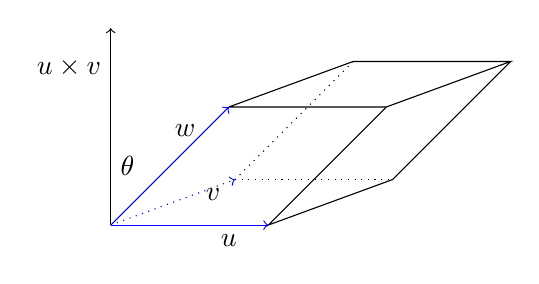
\begin{tikzpicture}
\draw[<-](0,2.5,0)--(0,0,0); 
\draw[blue,->](0,0,0)--(2,0,0); %% u 
\draw[blue,dotted,->](0,0,0)--(1,0,-1.5); %% v 
\draw[blue,->](0,0,0)--(1.5,1.5,0); %% w 
\draw[dotted](1,0,-1.5)--(3,0,-1.5);
\draw[dotted](1,0,-1.5)--(2.5,1.5,-1.5);
\draw(1.5,1.5,0)--(3.5,1.5,0)--(4.5,1.5,-1.5)--(2.5,1.5,-1.5)--(1.5,1.5,0);
\draw(3.5,1.5,0)--(2,0,0)--(3,0,-1.5)--(4.5,1.5,-1.5);
\node[left] at (0,2){$\vect{u} \times \vect{v}$};
\node[above right] at (0,0.5){$\theta$};
\node[below] at (1.5,0,0){$\vect{u}$};
\node[right] at (0.7,0,-1){$\vect{v}$};
\node[left] at (1.2,1.2,0){$\vect{w}$};
\end{tikzpicture}
\end{center}

Notice that the base of the parallelepiped is the parallelogram
determined by the vectors $\vect{u}$ and $\vect{v}$. Therefore, its area is equal to 
$\vectlength \vect{u}\times \vect{v} \vectlength $. The height of the parallelepiped
is $\vectlength \vect{w}\vectlength \cos \theta $ where $\theta $ is the angle
shown in the picture between $\vect{w}$ and $\vect{u}\times \vect{v}$.
The volume of this parallelepiped is the area of the base times
the height which is just
\begin{equation*}
\vectlength \vect{u}\times \vect{v}\vectlength \vectlength \vect{w}\vectlength \cos \theta =
\left( \vect{u}\times\vect{v}\right) \dotprod \vect{w}
\end{equation*}
This expression is known as the box product and is sometimes written as 
$\left[ \vect{u},\vect{v},\vect{w}\right] .$
\index{box product}You should consider what happens if you interchange the 
$\vect{v}$ with the $\vect{w}$ or the $\vect{u}$ with the $\vect{w}$.
You can see geometrically from drawing pictures that this merely introduces
a minus sign. In any case the box product of three vectors always equals
either the volume of the parallelepiped determined by the three vectors or
else $-1$ times this volume.

\begin{proposition}{The box product}{boxproduct}
Let $\vect{u}, \vect{v}, \vect{w}$ be three vectors in $\R^n$ that define a parallelepiped. Then the volume of the parallelepiped is the absolute value of the box product, given by 
\[
\left| \left(\vect{u}\times\vect{v}\right) \dotprod \vect{w} \right|
\]
\end{proposition}

Consider an example of this concept.

\begin{example}{Volume of a parallelepiped}{parallelepipedvolume}
Find the volume of the parallelepiped determined by the vectors
\begin{equation*}
\vect{u}
=
\begin{mymatrix}{r}
1 \\
2 \\
-5
\end{mymatrix}, 
\vect{v}
=
\begin{mymatrix}{r}
1 \\
3 \\
-6
\end{mymatrix}, 
\vect{w}
=
\begin{mymatrix}{r}
3 \\
2 \\
3
\end{mymatrix}
\end{equation*}
\end{example}

\begin{solution}
According to the above discussion, pick any two of these vectors, take the cross
product and then take the dot product of this with the third of these
vectors. The result will be either the desired volume or $-1$ times the desired
volume. Therefore by taking the absolute value of the result, we obtain the volume. 

We will take the cross product of $\vect{u}$ and $\vect{v}$. 
This is given by 
\begin{align*}
\vect{u} \times \vect{v}
&=
\begin{mymatrix}{r}
1 \\
2 \\
-5
\end{mymatrix}
\times
\begin{mymatrix}{r}
1 \\
3 \\
-6
\end{mymatrix}\\
&=((2)(-6)-(-5)(3))\vect{i}+((1)(-6)-(-5)(1))\vect{j}+((1)(3)-(2)(1))\vect{k} \\
&= 3\vect{i}+\vect{j}+\vect{k}
=
\begin{mymatrix}{r}
3 \\
1 \\
1
\end{mymatrix} 
\end{align*}

Now take the dot product of this vector with $\vect{w}$ which yields
\begin{eqnarray*}
(\vect{u} \times \vect{v}) \dotprod \vect{w}
&=&
\begin{mymatrix}{r}
3 \\
1 \\
1
\end{mymatrix}
\dotprod
\begin{mymatrix}{r}
3 \\
2 \\
3 
\end{mymatrix} \\
&=&\left( 3\vect{i}+\vect{j}+\vect{k}\right) \dotprod
 \left( 3\vect{i}+2\vect{j}+3\vect{k}\right) \\
&=&9+2+3 \\
&=&14
\end{eqnarray*}

This shows the volume of this parallelepiped is 14 cubic units.
\end{solution}

There is a fundamental observation which comes directly from the geometric
definitions of the cross product and the dot product.

\begin{proposition}{Order of the product}{orderofproduct}
Let $\vect{u},\vect{v}$, and $\vect{w}$ be vectors. Then $\left(
\vect{u}\times \vect{v}\right) \dotprod \vect{w}=\vect{u}\dotprod \left( \vect{v}\times \vect{w}
\right) .$
\end{proposition}

\begin{proof}This follows from observing that either 
$\left( \vect{u}\times \vect{v}\right) \dotprod \vect{w}$ and $\vect{u}\dotprod 
\left( \vect{v}\times \vect{w}\right) $ both give the volume of the parallelepiped or they both
give $-1$ times the volume.
\end{proof}

\begin{comment}
Recall that we can express the cross product as the determinant of a particular matrix. It turns out
that the same can be done for the box product. 
Suppose you have three vectors, $\vect{u}=\begin{mymatrix}{rrr}
a & b & c
\end{mymatrix}^T ,\vect{v}=\begin{mymatrix}{rrr}
 d & e & f
\end{mymatrix}^T ,$ and $\vect{w}=\begin{mymatrix}{rrr}
g & h & i
\end{mymatrix}^T .$ Then the box product $\vect{u}\dotprod \left(\vect{v}\times \vect{w}\right)$ is given by the following.
\begin{eqnarray*}
\vect{u}\dotprod \left(\vect{v}\times \vect{w}\right) &=&
\begin{mymatrix}{r}
a \\
b \\
c
\end{mymatrix} \dotprod \left|
\begin{array}{rrr}
\vect{i} & \vect{j} & \vect{k} \\
d & e & f \\
g & h & i
\end{array}
\right| \\
&=&a\left|
\begin{array}{rr}
e & f \\
h & i
\end{array}
\right| -b\left|
\begin{array}{rr}
d & f \\
g & i
\end{array}
\right| +c\left|
\begin{array}{rr}
d & e \\
g & h
\end{array}
\right| \\
&= &\det \begin{mymatrix}{rrr}
a & b & c \\
d & e & f \\
g & h & i
\end{mymatrix} 
\end{eqnarray*}

To take the box product, you can simply take the
determinant of the matrix which results by letting the rows be the
components of the given vectors in the order in which they occur
in the box product. 

This follows directly from the definition of the cross product given above
and the way we expand determinants. Thus the volume of a parallelepiped
determined by the vectors $\vect{u},\vect{v},\vect{w}$ is just the
absolute value of the above determinant.
\end{comment}


